\documentclass[11pt,a4paper]{article}
\usepackage[utf8]{inputenc}
\usepackage[british]{babel}
\usepackage[a4paper,margin=2.3cm]{geometry}
\usepackage{amsmath,amssymb}
\usepackage{graphicx}
\usepackage{tikz}
\usetikzlibrary{calc,angles,quotes,patterns}
\usepackage[most]{tcolorbox}
\usepackage{enumitem}
\usepackage{array}
\usepackage{titlesec}
\usepackage[hidelinks]{hyperref}

\definecolor{bandgreen}{RGB}{46,139,87}
\definecolor{bandblue}{RGB}{30,100,190}
\definecolor{bandamber}{RGB}{220,140,20}
\definecolor{bandpink}{RGB}{210,70,140}
\definecolor{bandpurple}{RGB}{110,50,160}

\newcounter{prob}
% \prob{label}{title}{source}
\newcommand{\prob}[3]{\par\bigskip\refstepcounter{prob}\label{#1}%
  \noindent\textbf{\theprob.\ #2}\hfill{\small\textit{#3}}\par\nopagebreak\smallskip}
\newcommand{\ans}[2]{\par\smallskip\noindent\textbf{\ref{#1}.}\ #2}

\newcommand{\band}[3]{%
  \clearpage
  \begin{tcolorbox}[colback=#1!12,colframe=#1,boxrule=1pt,arc=2pt]
  {\Large\bfseries\color{#1} #2}\hfill{\large #3}
  \end{tcolorbox}}

\newtcolorbox{diarynote}[1]{colback=black!4,colframe=black!45,boxrule=0.6pt,
  arc=2pt,fonttitle=\bfseries\small,title={#1},fontupper=\small}

\setlength{\parindent}{0pt}
\setlength{\parskip}{3pt}
\begin{document}

\begin{titlepage}
\centering
\vspace*{3cm}
{\Huge\bfseries The Ladies' Diary\par}
\vspace{0.4cm}
{\LARGE Third book\par}
\vspace{0.8cm}
{\Large Fifty-five problems, 1749--1776,\\ for readers from five to seventeen\par}
\vspace{2cm}
{\large\itshape Five times seven and seven times three\\
Add to my age, the sum will be\\
As many above six nines and four\\
As twice my years exceed a score.\par}
\vspace{0.3cm}
{\small Miss Maria Atkinson, question 391\par}
\vfill
{\large Working draft\par}
\end{titlepage}

\section*{A word before the problems}

In 1755 a Mr E.~P.\ asked Miss Maria Atkinson her age. She answered him in the Diary, in
rhyme, as an equation. Mr B.~Lydal solved it the next year and told her the answer, 18,
was ``a very good age for matrimony, Miss''. That is the Diary of the middle of the
century: teasing, public and mathematical.

This booklet takes fifty-five problems from the second volume of Thomas Leybourn's
collection of 1817. It covers questions 295 to 698, set from 1748 and answered from
1749 to 1776. The running heads of the volume name four editors in turn: Robert Heath,
Thomas Simpson, Edward Rollinson and Charles Hutton. Hutton appears first as a reader.
In 1764 a ``Mr C.~Hutton'' sends in an answer, and later he sets questions of his own.

Women still set questions in these years, though fewer than before. Seven of the four
hundred carry a woman's name or a woman's pen-name: Amanda, Rosamond, Miss Munlove,
Miss Maria Atkinson (twice), Miss T.~S---e and Miss S.~T. That is about one in sixty.
Another ten are signed Miss Ann Nicholls, a name the Diary spells three ways. Most of
them are astronomy: when the Sun rises at two towns, or the hour at which two stars
stand in one vertical circle. Leybourn's index says who wrote them: ``Nichols, Ann.
(Mr.~W.~Wales).'' William Wales was an astronomer, later with Cook on his second
voyage. The index gives him four other pen-names as well. A woman's name on a question
did not always mean a woman. Three of the Nicholls questions are in this booklet,
labelled with both names.\footnote{Questions 462, 475 and 567. Counted the same way,
the first volume has about one question in thirty from a woman. Almost all of them
come from 1709--1724, when the rate was about one in ten. The third volume has about
one in eighty, and the fourth about one in two hundred.}

Children wrote in too. ``Master Dickey'' set a question about packs of cards, and
``Master Billy Branch, of Rochester'' answered it. Master John Birks, ``a Tyro, at
Gosberton School'', answered a question about a square field. Two boys from the
Mathematical Academy at Bristol, J.~Paty and J.~Osborne, are described as ``youths of
about 13 years of age''. Paty set the question about the cow and her calves.

One question came from further off. In 1769 the Diary printed a theorem that Pierre de
Fermat had sent to John Wallis, ``which was never yet publicly answered''. It is
problem~\ref{u-fermat}.

\subsection*{How to read the labels}

\textit{Q462} means question~462 in Leybourn's volume~II, in modern words. \textit{After
Q462} means the problem has been retold. It may have new numbers for younger readers,
or metres in place of yards, poles and chains, or pounds and pence in place of
shillings. The idea is always the Diary's. Where a retelling changes the answer, the
answer given is for the retelling. Two problems keep their guineas, shillings and
pence, because they depend on them.

\subsection*{The bands}

\begin{center}
\begin{tabular}{>{\bfseries}l l l r}
\color{bandgreen}Green  & ages 5--8   & sharing, counting, balancing          & 3\\
\color{bandblue}Blue    & ages 8--11  & remainders, digits, shares            & 5\\
\color{bandamber}Amber  & ages 11--14 & first algebra, money, patterns        & 10\\
\color{bandpink}Pink    & ages 14--16 & GCSE: interest, probability, triangles & 16\\
\color{bandpurple}Purple & ages 16--17 & A-level: proof, optimisation, numbers & 21\\
\end{tabular}
\end{center}

Answers are at the back. When the Diary or its readers went wrong, a small grey box
says so.

\subsection*{How this edition was made}
This edition was prepared with the assistance of Claude, an AI model made by Anthropic.
Under the editor's direction, Claude drafted the retellings, solutions, notes and
introduction, recomputed every answer, worked from the Internet Archive's machine-read
text of the source, and typeset the text. Selection, editorial decisions and final
responsibility for the text are the editor's.

%================ GREEN ================
\band{bandgreen}{Green}{ages 5--8}

\prob{g1}{Red and blue}{after Q335, by Master Dickey}
On a balance, 10 red counters and 3 blue counters weigh exactly the same as 4 red
counters and 9 blue counters. Which is heavier, a red counter or a blue one?
\textit{Hint: take the same counters off both sides.}

\prob{g2}{The little orchard}{after Q352, by Mr Randles}
In an orchard, half the trees are apple trees and a quarter are pear trees. The other 3
are cherry trees. How many trees are there?

\prob{g3}{The cow and her calves}{after Q584, by Master J.~Paty}
A calf is born. When she is two years old she has a calf of her own, and then one more
every year. Every calf does the same. Draw the cows year by year. How many are there
after six years?

%================ BLUE ================
\band{bandblue}{Blue}{ages 8--11}

\prob{b1}{Always one short}{Q296, by Amanda}
Find the smallest number that leaves 1 when divided by 2, leaves 2 when divided by 3, 3
when divided by 4, 4 when divided by 5, and 5 when divided by 6.

\prob{b2}{Miss Atkinson's age}{Q391, by Miss Maria Atkinson}
Five times seven and seven times three, added to her age, come to as much above six
nines and four as twice her age is above twenty. How old is she?

\prob{b3}{Old John's windfall}{Q475, by ``Miss Ann Nicholls'' (William Wales)}
Old John receives a sum of money. He pays his debts, \pounds94 in all. He lends half of what
is left to a friend, and spends a fifth of what was left after the debts on himself and
Joan. He finds he still has a tenth of the sum he received. How much did he receive?

\prob{b4}{The guineas at hazard}{Q338, by William Leighton}
A wins a number of guineas from B at dice. The number has three digits, and the digits
go up or down in equal steps. Divide the number by the sum of its digits and you get 48.
Take away 198 and its digits are reversed. How many guineas did A win?

\prob{b5}{Fifteen hundred pounds}{Q421, by Juvenis}
Three men share \pounds1,500. A's share is to B's as 4 is to 3, and C has \pounds70 more than A.
What does each man get?

%================ AMBER ================
\band{bandamber}{Amber}{ages 11--14}

\prob{a-courier}{The courier's four days}{Q377, by Miss Maria A---i---s---n}
Three towns lie on one road. $A$ is 136 miles from $B$, and $B$ is 104 miles from $C$.
A courier rides from $A$ to $B$ in two days and from $B$ to $C$ in two more. Each day he
rides the same number of miles less than the day before. How far does he ride on each
day?

\prob{a-height}{Height, years and fortune}{Q434, by Miss T.~S---e}
Her height in inches is three times her age in years. Her fortune in pounds is the sum
of the squares of the two. Height, age and fortune together come to 4,494. Find all
three.

\prob{a-partners}{Two partners}{Q462, by ``Miss Ann Nichols'' (William Wales)}
Two partners, $A$ and $B$, make \pounds400 in a venture. $A$ put in \pounds81 more than $B$. $B$'s
share of the profit is \pounds190. Profits are shared in proportion to what each put in. How
much did each put in?

\prob{a-drover}{The drover's sheep}{after Q463, by Miss S.~T.}
A drover buys some sheep for \pounds46. He sells a third of them at \pounds1 each, a quarter at 90p
each and the rest at 80p each, and makes \pounds7.50 profit. How many sheep did he buy?

\prob{a-any}{Any two parts}{Q476, by John Hampson}
Find a number with this property: however you split it into two unequal parts, the
larger part plus the square of the smaller equals the smaller part plus the square of
the larger.

\prob{a-paving}{Paving and fencing}{after Q436, by John Brickland of Oxford}
A garden is an equilateral triangle. Paving it costs \pounds8 a square metre, and fencing its
three sides costs \pounds84 a metre. The two bills are the same. How long is each side?

\prob{a-interest}{All the same number}{after Q365, by John Williams}
Some money is lent at simple interest. The number of pounds lent, the rate of interest
per cent and the number of years are all the same number. The interest comes to half
the sum lent. Find the number.

\prob{a-barter}{John and Hodge}{after Q406, by Rusticus}
John brings sheep to market and Hodge brings pigs and geese. They swap: John's sheep
for all of Hodge's pigs and geese. A sheep is worth one pig and one goose together, and
a goose is worth \pounds2. There are 16 more pigs and geese together than sheep, and 10 more
geese than pigs. The pigs and geese together are worth \pounds100. How many of each are
there, and what is a pig worth?

\prob{a-horse}{The horse that cost too much}{after Q376, by Rusticus}
A man buys a horse for \pounds26, keeps it for a while and sells it for \pounds60. Even so, he
loses half the price he paid plus a quarter of what the horse cost him to keep. What
did the keep cost, and how much did he lose?

\prob{a-cows}{Forty years of cows}{Q584, by Master J.~Paty}
A cow has a she-calf at the age of two and one more every year after. Every one of her
brood does the same. How many calves spring from the old cow and her brood in 40 years?
\textit{Hint: count the new calves year by year and look for the pattern.}

%================ PINK ================
\band{bandpink}{Pink}{ages 14--16}

\prob{p-poultry}{Geese, ducks and chickens}{Q308, by Upnorensis}
A lady pays twice as much for a goose as for a duck, and twice as much for a duck as for
a chicken. The birds cost \pounds1 13s 4d in all, that is 400 pence. The squares of the
numbers of geese, ducks and chickens add up to 326. How many of each did she buy, and
at what prices? In old money a penny could be split into four farthings.

\prob{p-halfpence}{Twelve halfpennies}{Q416, by Thomas Moss}
Twelve coins are tossed. Those that come up heads are taken away, and the rest are
tossed again, and so on until every coin has come up heads. After how many rounds is it
an even chance that all the coins have gone? \textit{Hint: one coin survives $n$ rounds
with probability $\left(\tfrac12\right)^n$.}

\prob{p-interest}{Simple against compound}{Q485, by Hugh Brown}
$A$ and $B$ each borrow \pounds400 for the same time at the same rate. $A$ pays compound
interest and owes \pounds463.05 at the end. $B$ pays simple interest and owes \pounds460. Find the
rate and the time.

\prob{p-annuity}{Five years and ten}{Q569, by Richard Gibbons}
A sum is paid into an account at the end of every year and earns compound interest.
After 5 years the account holds \pounds500. After 10 years it holds \pounds1,100. Find the rate of
interest and the yearly payment.

\prob{p-tortoise}{The tortoise and the hare}{Q435, by Patrick O'Cavanah of Dublin}
A hare runs 4 furlongs in the first minute of a race, then 2 in the second, 1 in the
third, and so on, halving every minute. A tortoise crawls a quarter of a furlong every
minute. When does the tortoise catch the hare?

\prob{p-lens}{The square in the lens}{Q394, by W.~Kingston}
Two circles each 50\,cm across have their centres 30\,cm apart. Find the side of the
largest square that fits in the region common to both.
\begin{center}
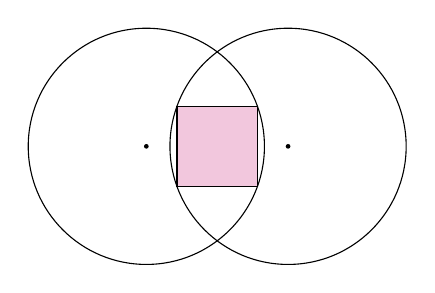
\begin{tikzpicture}[scale=0.06]
\draw (-15,0) circle (25); \draw (15,0) circle (25);
\fill[bandpink!30] (-8.508,-8.508) rectangle (8.508,8.508);
\draw (-8.508,-8.508) rectangle (8.508,8.508);
\fill (-15,0) circle (0.5); \fill (15,0) circle (0.5);
\end{tikzpicture}
\end{center}

\prob{p-1315}{Product, product and height}{Q353, by Taptinos}
In a triangle, the two sides multiplied together make 195. The perpendicular from the
top to the base is 12, and it cuts the base into two parts that multiply to 45. Find the
three sides.

\prob{p-incircle}{Through the centre to the far leg}{Q351, by Taptinos}
In a right-angled triangle $ABC$, with the right angle at $B$, the distance from $A$ to
the centre of the inscribed circle is 4\,m. The same line, continued 2\,m further, meets
the leg $BC$. Find the sides.

\prob{p-fountain}{The fountain in the garden}{after Q386, by Timothy Doodle}
A rectangular garden has an area of 4,840\,m$^2$. Inside it is a round fountain. The
edge of the fountain is 60, 52, 28 and 40\,m from the four corners, taken in order round
the garden. How wide is the fountain, and what are the length and breadth of the garden?
\textit{Hint: start with the fountain.}

\prob{p-oak}{The oak and the square field}{after Q370, by Joseph Hilditch}
An oak stands outside a square field. Its distances to the three corners it can see are
78\,m, 59.161\,m and 78\,m, in that order. How big is the field?

\prob{p-echo}{The gun and the echo}{after Q567, by ``Miss Anna Nicholls'' (William Wales)}
Walking on the shore, I see the flash of a gun bearing SE by E. Seven seconds later I
hear the report, and four seconds after that I hear its echo from a castle bearing
SW by W. Sound travels 340\,m a second. How far am I from the castle, and how far is the
castle from the gun? \textit{Each compass point is $11\tfrac14^\circ$.}

\prob{p-cistern}{The cistern}{after Q342, by Stephen Hodges the younger}
A cistern is a box with a rectangular top. Its length and breadth add up to 84\,cm, and
the diagonal of the top is 60\,cm. Its breadth is to its depth as 25 is to 7. Find its
three dimensions.

\prob{p-steeple}{Three looks at a steeple}{after Q478, by W.~Chapman}
I measure the angle of elevation of a steeple's top. I walk 60\,m nearer on level
ground, and the angle is now the complement of the first. I walk 20\,m nearer still,
and the angle is exactly double the first. How tall is the steeple?

\prob{p-squares}{Two numbers, three squares}{Q491, by John Hampson}
Find two whole numbers, neither of them a square, whose product is a square, and such
that the product plus the square of either number is also a square.

\prob{p-median}{The median and the base}{Q495, by W.~Spicer}
Two sides of a triangle are 30 and 40. The line from the angle between them to the
middle of the third side is drawn. The product of this line and the third side is as
large as possible. Find both.

\prob{p-chords}{A line through the crossing}{Q570, by Robert Butler}
Two circles have radii 6\,cm and 8\,cm, and their centres are 10\,cm apart. Through one
of the points where they cross, draw a straight line 19\,cm long with its ends on the two
circles. How is the line divided at the crossing point?

%================ PURPLE ================
\band{bandpurple}{Purple}{ages 16--17}

\prob{u-rosamond}{Seven more than itself}{Q305, by Rosamond}
The aliquot parts of a number are its divisors smaller than itself. Find the smallest
number whose aliquot parts add up to 7 more than the number.

\prob{u-servants}{Placing the servants}{Q298, by Miss Munlove}
A gentleman places his servants in a row: one at a time, or two, or three, and so on up
to all of them. Each choice of servants and each order counts as a different way. He
finds 960,799 ways in all. How many servants does he keep?

\prob{u-ages}{A wife and a daughter}{Q393, by G.~Brownbridge}
Two ages, $x$ and $z$, satisfy $x^3z + xz^3 = 546{,}560$ and $x^4 + z^4 = 1{,}086{,}992$.
Find them.

\prob{u-annuity}{Ten years against twenty}{Q379, by John Morland}
Two people share an annuity of \pounds100 a year for 30 years. $A$ takes every payment for the
first 10 years and $B$ every payment for the last 20. The two shares are worth the same
today. Find the rate of compound interest.

\prob{u-centroid}{Three perpendiculars}{Q409, by H.~Watson}
A triangle has sides 16, 20 and 24. From a point inside it, perpendiculars are dropped to
the three sides. Where must the point be for the product of the three perpendiculars to
be as large as possible? What is the product?

\prob{u-watering}{The watering place}{after Q410, by Walter Trott}
A field is a right-angled triangle. A watering place inside it is 38\,m from the
right-angled corner and 62\,m and 50\,m from the other two corners. How large can the
field be?

\prob{u-diagonals}{Equal diagonals}{after Q425, by James Beresford}
A field has four straight sides of 25, 35, 31 and 19\,m, in that order, and its two
diagonals are equal. Find its area. \textit{Hint: compare $25^2 + 31^2$ with $35^2 +
19^2$.}

\prob{u-quad}{Three to five}{after Q408, by R.~Young of Chester}
A field has four sides of 90, 100, 110 and 120\,m. A diagonal divides it so that the
triangle on the two shortest sides is to the other triangle as 3 is to 5. Find the area
of the field.

\prob{u-heron}{Area, perimeter and squares}{Q488, by Richard Mallock}
A triangle has area 126 and perimeter 54, and the squares of its sides add up to 1,010.
Find the sides.

\prob{u-reciprocal}{By a quadratic only}{Q521, by Joseph Walker}
Solve $(x+1)(x^2+1)(x^3+1) = 30x^3$, using no equation harder than a quadratic.

\prob{u-harmonic}{Three in harmonic proportion}{Q537, by W.~Toft}
Three numbers are in harmonic proportion: their reciprocals go up in equal steps. Their
sum is 191 and their product is 254,016. Find them.

\prob{u-isosceles}{The line from the top}{Q439, by W.~Bevil}
An isosceles triangle has base 100 and equal sides 60. A line is drawn from the top to the
base. The product of this line and the two parts of the base is as large as possible.
Find the line and the two parts.

\prob{u-fermat}{Fermat's question to Wallis}{Q606, by Monsieur Fermat}
$AB$ is the diameter of a semicircle. On the other side of $AB$, perpendiculars $AD$
and $BC$ are drawn, each equal to the chord of a quarter of the circle, that is
$AB/\sqrt2$. $E$ is any point on the semicircle. $ED$ and $EC$ cut $AB$ at $O$ and $V$.
Prove that $BO^2 + AV^2 = AB^2$.
\begin{center}
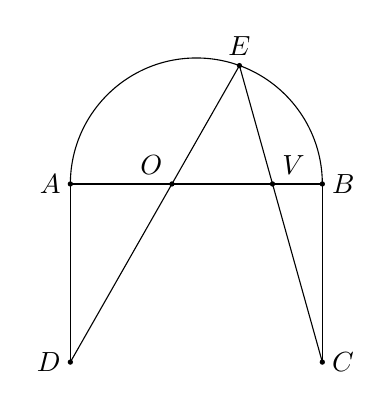
\begin{tikzpicture}[scale=0.8]
\coordinate (A) at (-2,0); \coordinate (B) at (2,0);
\coordinate (D) at (-2,-2.828); \coordinate (C) at (2,-2.828);
\coordinate (E) at (0.684,1.879);
\coordinate (O) at (-0.387,0); \coordinate (V) at (1.209,0);
\draw (2,0) arc (0:180:2);
\draw (A)--(B); \draw (A)--(D); \draw (B)--(C);
\draw (E)--(D); \draw (E)--(C);
\foreach \p/\q in {A/left,B/right,C/right,D/left,E/above,O/above left,V/above right}
  \fill (\p) circle (1.2pt) node[\q]{$\p$};
\end{tikzpicture}
\end{center}

\prob{u-euler}{The midpoints of the diagonals}{Q380, by W.~T---t}
In any quadrilateral, the squares of the two diagonals, together with the square of
twice the line joining their midpoints, equal the sum of the squares of the four sides.
Prove it.

\prob{u-fraction}{A fraction and its reciprocal}{Q585, by Jeremiah Ainsworth}
Find a fraction which, taken from its reciprocal, leaves a perfect square.

\prob{u-equilateral}{The greatest equilateral field}{after Q396, by Thomas Moss}
Three trees stand 100, 120 and 160\,m from one another. An equilateral triangular field
is to be laid out with one tree on each of its sides. How large can the field be?

\prob{u-whitfield}{Where should Whitefield preach?}{after the prize question, answered 1751, by John Turner of Brompton}
Three towns $A$, $B$ and $C$ are 7 miles from $A$ to $B$, 8 from $B$ to $C$ and 10 from
$C$ to $A$. Four thousand people live in $A$, two thousand in $B$ and three thousand in
$C$. All of them will walk to hear the preacher George Whitefield. Where should he
preach so that the total distance walked, and so the shoe leather worn, is least?

\prob{u-urn}{The urn on the column}{after Q615, by John Chipchase}
In Stockton market place a column carries an urn 1.5\,m tall. To a person whose eye is
1.6\,m above the ground, standing 10\,m from the foot of the column, the urn looks as
large as it possibly can. How tall is the column?

\prob{u-trees}{Four trees in a hedge}{after Q313, by John Landen}
Four tall trees stand in a straight hedge. The first is 60\,m from the second, the
second 20\,m from the third, and the third 40\,m from the fourth. Where must I stand so
that the three gaps between them look equally wide?

\prob{u-sheep}{The fewest squares}{after Q426, by W.~Spicer}
A man spends \pounds1,200 on sheep of three sorts, at \pounds9, \pounds12 and \pounds15 each. He buys them in
such numbers that the sum of the squares of the three numbers is as small as possible.
How many of each does he buy?

\prob{u-mean}{A mean proportional}{Q437, by Thomas Moss}
A triangle has base $AB = 70$ and sides $AC = 50$, $BC = 40$. Draw a line from $C$ to a
point $P$ of the base so that $CP$ is a mean proportional between $AP$ and $PB$, that is
$CP^2 = AP\times PB$. Where is $P$?

%================ ANSWERS ================
\clearpage
\section*{Answers}

\subsection*{\color{bandgreen}Green}
\ans{g1}{They weigh the same. Take 4 red and 3 blue counters off each side. That leaves
6 red on one side and 6 blue on the other, and they still balance. In the Diary the
question was set by Master Dickey and answered by Master Billy Branch of Rochester:
``the value of a pack of knaves is only a pack of cards''.}
\ans{g2}{12 trees: 6 apple, 3 pear and 3 cherry. The cherry trees are the quarter that
is left over.}
\ans{g3}{13. Year by year the herd is 1, 1, 2, 3, 5, 8, 13. Each year's number is the
sum of the two before it.}

\subsection*{\color{bandblue}Blue}
\ans{b1}{59. Each remainder is one less than the divisor, so the number plus 1 divides
exactly by 2, 3, 4, 5 and 6. The smallest such number is 60.}
\ans{b2}{18. Her age plus 56 is as far above 58 as twice her age is above 20. So her
age less 2 equals twice her age less 20. Mr B.~Lydal answered: ``A very good age for
matrimony, Miss.''}
\ans{b3}{\pounds141. After the debts \pounds47 is left. He lends \pounds23.50 and spends \pounds9.40, which
leaves \pounds14.10, a tenth of \pounds141.}
\ans{b4}{432. Its digits 4, 3, 2 add up to 9, and $432 = 48\times9$. Also
$432 - 198 = 234$.}
\ans{b5}{A gets \pounds520, B \pounds390 and C \pounds590. Split A's share into 4 equal parts and B's
into 3. Then C has 4 parts and \pounds70, so 11 parts and \pounds70 make \pounds1,500, and one part is
\pounds130.}

\subsection*{\color{bandamber}Amber}
\ans{a-courier}{72, 64, 56 and 48 miles. If the daily drop is $d$, the first two days
add to $136$ and the last two to $136 - 4d$. So $4d = 32$.}
\ans{a-height}{She is 21, she is 63 inches tall, and her fortune is \pounds4,410. If her age
is $y$, then $y + 3y + y^2 + 9y^2 = 4494$, that is $10y^2 + 4y - 4494 = 0$.}
\ans{a-partners}{$A$ put in \pounds850.50 and $B$ \pounds769.50 (the Diary's \pounds850 10s and
\pounds769 10s). $A$'s profit is \pounds210 and $B$'s is \pounds190, so $A$'s stock is to $B$'s as 21 to
19. The difference, \pounds81, is 2 parts in 40, so one part is \pounds40.50. The answer was
printed under the name Amaryllis.}
\ans{a-drover}{60 sheep: 20 sold at \pounds1, 15 at 90p and 25 at 80p. The takings are
\pounds53.50, which is \pounds7.50 more than the \pounds46 they cost. The number must divide by 3 and by
4, so try multiples of 12.}
\ans{a-any}{1. If the parts are $a$ and $b$, then $a + b^2 = b + a^2$ gives
$(a - b)(a + b - 1) = 0$. The parts are unequal, so $a + b = 1$.}
\ans{a-paving}{$42\sqrt3 \approx 72.75$\,m. Paving costs $8\times\tfrac{\sqrt3}{4}s^2$
and fencing $84\times3s$. Setting them equal gives $s = 126/\sqrt3$.}
\ans{a-interest}{$\sqrt{50}\approx7.07$: \pounds7.07 at 7.07 per cent for 7.07 years. The
interest is $n\times\tfrac{n}{100}\times n$, and this must be $\tfrac n2$, so $n^2 = 50$.}
\ans{a-barter}{8 pigs worth \pounds8 each, 18 geese and 10 sheep worth \pounds10 each. If there
are $p$ pigs worth \pounds$x$, then $px + 2(p + 10) = 100$. There are $2p - 6$ sheep, each worth
$x + 2$. Trying whole numbers, $p = 8$ and $x = 8$ fit both.}
\ans{a-horse}{The keep cost \pounds$62\tfrac23$ and he lost \pounds$28\tfrac23$. His total outlay
was $26 + k$ and he got back 60, so $26 + k - 60 = 13 + \tfrac k4$. This gives
$\tfrac34k = 47$.}
\ans{a-cows}{The new calves each year are 0, 1, 1, 2, 3, 5, 8, \dots: from the third
year on, each year's number is the sum of the two before. These are the Fibonacci
numbers. Over 40 years they add up to 165,580,140 calves. With the old cow herself the
herd is 165,580,141. William Spicer's answer in the Diary is the same.}

\subsection*{\color{bandpink}Pink}
\ans{p-poultry}{There are three answers.
\begin{itemize}[nosep]
\item 13 geese at 1s 8d, 11 ducks at 10d and 6 chickens at 5d.
\item 9 geese at 2s 1d, 7 ducks at 1s $\tfrac12$d and 14 chickens at 6$\tfrac14$d.
\item 11 geese, 3 ducks and 14 chickens, at the same prices as the second.
\end{itemize}
Only four sets of three whole numbers have squares adding to 326: $\{1,10,15\}$,
$\{3,11,14\}$, $\{6,11,13\}$ and $\{7,9,14\}$. If a chicken costs $c$ pence, then
$c\,(4g + 2d + h) = 400$. So $4g + 2d + h$ must divide 1,600, the bill in farthings. Try
each set in each order.}
\ans{p-halfpence}{5. A coin is still in play after $n$ rounds with probability
$\left(\tfrac12\right)^n$. So all twelve have gone with probability
$\left(1 - \tfrac1{2^n}\right)^{12}$. This is 0.461 after 4 rounds and 0.683 after 5.
Edward Rollinson's answer put the exact even chance at about 4.16 rounds, ``4 being a
small matter too little, and 5 considerably too great''.}
\ans{p-interest}{5 per cent for 3 years. From $1.15 = 1 + rt$ and
$1.157625 = (1+r)^t$, try $t = 3$: $1.05^3 = 1.157625$.}
\ans{p-annuity}{About 3.71 per cent, and \pounds92.84 a year (the Diary's \pounds92 16s 10d and a
fraction). After 10 years the account holds the first five years' \pounds500, grown for five
more years, plus another \pounds500. So $1100 = 500(1+i)^5 + 500$, and $(1+i)^5 = 1.2$. The
first answer printed came from two boys at the Mathematical Academy in Bristol, J.~Paty
and J.~Osborne, ``youths of about 13 years of age''.}
\ans{p-tortoise}{A tiny moment before 32 minutes. After $t$ minutes the hare has run
$8\left(1 - 2^{-t}\right)$ furlongs and the tortoise $\tfrac t4$. They meet when
$t = 32 - 32\times2^{-t}$, which is less than half a millionth of a second short of 32
minutes. The hare never reaches 8 furlongs. Mr B.~Lydal's answer: 32 minutes,
``extremely near''.}
\ans{p-lens}{About 17.02\,cm. By symmetry the square is centred midway between the
centres, with half-side $x$. Its far corners lie on the circles, so
$(15 + x)^2 + x^2 = 25^2$, that is $x^2 + 15x - 200 = 0$, and $x \approx 8.508$.}
\ans{p-1315}{13, 15 and 14: the base is cut into 9 and 5. Write $p$ and $q$ for the
parts of the base. Then $(p^2 + 144)(q^2 + 144) = 195^2$ and $pq = 45$, which give
$p^2 + q^2 = 106$. So $p + q = 14$ and $p - q = 4$.}
\ans{p-incircle}{$AB = 12/\sqrt5 \approx 5.37$\,m, $BC = 16/\sqrt5 \approx 7.16$\,m and
$AC = 20/\sqrt5 \approx 8.94$\,m, a 3--4--5 triangle. Let $\alpha$ be half the angle at
$A$. The line from $A$ through the centre bisects that angle, and it meets $BC$ 6\,m
from $A$, so $AB = 6\cos\alpha$. The centre is 4 from $A$ and lies $r = 4\sin\alpha$
from both legs, so also $AB = 4\cos\alpha + 4\sin\alpha$. Hence $\tan\alpha = \tfrac12$,
and $\tan A = \tfrac43$.}
\ans{p-fountain}{The fountain is 20\,m across, and the garden is about 95.0\,m by
50.9\,m. For any point inside a rectangle, the squares of its distances to opposite
corners have equal sums. With radius $r$,
$(60 + r)^2 + (28 + r)^2 = (52 + r)^2 + (40 + r)^2$, so $r = 10$. The centre is then 70,
62, 38 and 50\,m from the corners, and the area fixes the rest. One other rectangle,
about 87.1\,m by 55.6\,m, fits the numbers too. In it the fountain pokes through the
wall, so it is not ``within'' the garden.}
\ans{p-oak}{The field is 24\,m square, 576\,m$^2$. The oak is equally far from the two
outer corners, so it lies on the diagonal through the near corner, and the angle at
that corner between the oak and either side is $135^\circ$. The cosine rule gives
$78^2 = 59.161^2 + s^2 + 2(59.161)s\cos45^\circ$. Note that $59.161^2 \approx 3500$. One of
the answers printed in the Diary came from Master John Birks, ``a Tyro, at Gosberton
School''.}
\ans{p-echo}{About 895\,m to the castle, and 2,845\,m from the castle to the gun. The gun
is $7\times340 = 2380$\,m away. The echo travels gun--castle--me in 11 seconds,
3,740\,m. The bearings are $112\tfrac12^\circ$ apart. Write $c$ for my distance from the
castle; the cosine rule gives $(3740 - c)^2 = 2380^2 + c^2 - 2(2380)c\cos112\tfrac12^\circ$.
The equation is linear in $c$. In the Diary's feet, with sound at 1,142 feet a second,
William Spicer found 3,005.5 and 9,556.5 feet.}
\ans{p-cistern}{48\,cm long, 36\,cm broad and 10.08\,cm deep. From $l + b = 84$ and
$l^2 + b^2 = 3600$ we get $lb = 1728$, so $l$ and $b$ are 48 and 36. The depth is
$\tfrac7{25}\times36$. Joseph Orchard's answer also worked out the other reading, with the
diagonal running down the side of the cistern.}
\ans{p-steeple}{$\sqrt{5500} \approx 74.2$\,m. Let the foot be $B$ and the three stations
$C$, $D$, $E$, nearest last. The angle at $E$ is twice that at $C$, so triangle $CEA$ is
isosceles and $EA = EC = 80$. The first two angles are complementary, so
$h^2 = BC\times BD$. With $BE = y$: $(y + 80)(y + 20) = 6400 - y^2$, so $y = 30$. The first
station is 110\,m away.}
\ans{p-squares}{18 and 32 are the smallest. Their product is $576 = 24^2$, and
$576 + 18^2 = 30^2$ and $576 + 32^2 = 40^2$. Richard Mallock's method drops the
perpendicular to the hypotenuse of a 3--4--5 triangle. It cuts the hypotenuse into
$\tfrac95$ and $\tfrac{16}5$; multiply both by 10.}
\ans{p-median}{The angle between the given sides is a right angle. The third side is 50,
the median 25, and their product 1,250. For a median $m$ to a side $c$,
$4m^2 + c^2 = 2\times30^2 + 2\times40^2 = 5000$, a fixed sum. The product $(2m)c$ of two
numbers with a fixed sum of squares is largest when they are equal.}
\ans{p-chords}{Either 9.16\,cm in the larger circle and 9.84\,cm in the smaller, or
15.17\,cm and 3.83\,cm. Drop perpendiculars from the two centres to the line. They bisect
the two chords, so the whole line is twice the distance between their feet, which is
$2\times10\cos\phi$, where $\phi$ is the angle between the line and the line of centres.
So $\cos\phi = 0.95$. The radii 6, 8 and the distance 10 make a right angle at the
crossing point, which makes the rest quick. William Cole's answer in the Diary gives
both pairs.}

\subsection*{\color{bandpurple}Purple}
\ans{u-rosamond}{196. Its aliquot parts are 1, 2, 4, 7, 14, 28, 49 and 98, which add up
to 203. The sum of all divisors must be odd, which happens only when the number is a
square or twice a square, so few numbers need checking. Rosamond's question also asked
for amicable numbers, each the sum of the other's aliquot parts (see the first book,
problem ``Each made of the other's parts''). John Landen's answer gives 220 and 284,
17,296 and 18,416, and 9,363,584 and 9,437,056, with the rule that produces them. He
credits the rule to Descartes. It goes back to Th\=abit ibn Qurra in the ninth
century.}
\ans{u-servants}{Strictly, no number works. With $n$ servants the number of ordered
choices is $n + n(n-1) + n(n-1)(n-2) + \dots + n!$. That is 13,699 for 7 servants,
109,600 for 8 and 986,409 for 9. The Diary's answer, 7, came from a formula in Stone's
\textit{Mathematical Dictionary} that allows a servant to be used more than once:
$7 + 7^2 + \dots + 7^7 = 960{,}799$. See the grey box.}
\ans{u-ages}{32 and 14. Put $p = xz$ and $s = x^2 + z^2$. Then $ps = 546{,}560$ and
$s^2 - 2p^2 = 1{,}086{,}992$. Eliminating $s$ gives a quadratic in $p^2$, with
$p = 448$ and $s = 1220$. Then $(x+z)^2 = 2116$ and $(x-z)^2 = 324$.}
\ans{u-annuity}{About 4.93 per cent. Let $u$ be the value today of \pounds1 due in 10 years.
$A$'s share is worth $(1 - u)$ times a fixed amount, and $B$'s is worth $(u - u^3)$ times
the same. Equal shares give $u^3 - 2u + 1 = 0$, that is $(u - 1)(u^2 + u - 1) = 0$. So
$u = \tfrac{\sqrt5 - 1}{2}$, and $(1 + i)^{10} = \tfrac{1+\sqrt5}{2}$, the golden ratio.
At that rate the whole annuity is worth about \pounds1,550 today.}
\ans{u-centroid}{At the centroid, where the medians meet. A perpendicular to side $a$
is $2[PBC]/a$, so the product is largest when $[PBC]\,[PCA]\,[PAB]$ is. The three areas
add up to the whole triangle, so their product is largest when they are equal. The
perpendiculars are then a third of the heights: 6.614 to the side 16, 5.292 to 20 and
4.410 to 24. Their product is about 154.3.}
\ans{u-watering}{2,880\,m$^2$. Call the right-angled corner $B$, the watering place $D$, and
the corners $A$ and $C$, with $AD = 62$ and $CD = 50$. Patrick O'Cavanah's answer slides
triangle $ABD$ along $AB$, so that $A$ goes to $B$ and $D$ to a point $E$. Then
$DE = AB$, $BE = 62$, and $DE$ is perpendicular to $BC$. So the quadrilateral $BDCE$ has
the same area as the field, $\tfrac12 DE\times BC$. Its sides are 38, 50, $CE$ and 62,
where $CE^2 = 62^2 - 38^2 + 50^2$, so $CE = 70$. A quadrilateral with given sides is
largest when it lies in a circle. Then Ptolemy's theorem gives
$DE\times BC = 38\times70 + 50\times62 = 5760$.}
\ans{u-diagonals}{About 718\,m$^2$. Since $25^2 + 31^2 = 35^2 + 19^2$, the diagonals are
perpendicular. The area of such a quadrilateral is half the product of the diagonals,
here $\tfrac12d^2$. Write the four pieces of the diagonals as $a, b, c, e$. Then
$a^2 + b^2 = 25^2$, $b^2 + c^2 = 35^2$, $c^2 + e^2 = 31^2$ and $a + c = b + e$. Solving
gives $d \approx 37.90$\,m. The Diary's answer, in perches, was 4 acres 1 rood
$38\tfrac14$ perches, the same area.}
\ans{u-quad}{About 10,560\,m$^2$. Let the diagonal be $x$. By Heron's formula the two
triangles have areas
$\tfrac14\sqrt{(190^2 - x^2)(x^2 - 10^2)}$ and $\tfrac14\sqrt{(230^2 - x^2)(x^2 - 10^2)}$.
The ratio $3:5$ gives $25(190^2 - x^2) = 9(230^2 - x^2)$, so $x \approx 163.2$\,m. The
answer in the Diary was 10 acres 2 roods $9\tfrac12$ perches, with chains for sides.}
\ans{u-heron}{13, 20 and 21. The sides are the roots of $t^3 - 54t^2 + 953t - 5460 = 0$.
Their sum is 54. The sum of their products in pairs is $\tfrac12(54^2 - 1010) = 953$.
Heron's formula with $s = 27$ gives $(27 - a)(27 - b)(27 - c) = 126^2/27 = 588$, and
expanding that fixes the product $abc = 5460$.}
\ans{u-reciprocal}{$x = \tfrac{3\pm\sqrt5}{2}$, about 2.618 or 0.382. Multiplied out,
the equation is $x^6 + x^5 + x^4 - 28x^3 + x^2 + x + 1 = 0$. The coefficients read the
same backwards, so divide by $x^3$ and put $z = x + \tfrac1x$:
$z^3 + z^2 - 2z - 30 = 0$, that is $(z - 3)(z^2 + 4z + 10) = 0$. The quadratic factor has
no real roots, so $x + \tfrac1x = 3$. The two answers are the squares of the golden ratio
and of its reciprocal.}
\ans{u-harmonic}{72, 63 and 56. For the middle number $y$, $y(x + z) = 2xz$. With
$x + z = 191 - y$ and $xz = 254016/y$, this becomes $y^2(191 - y) = 508{,}032$, and
$y = 63$. Check: $\tfrac1{72}, \tfrac1{63}, \tfrac1{56}$ go up by $\tfrac1{504}$ each time.}
\ans{u-isosceles}{The line is $60/\sqrt3 \approx 34.64$, and it cuts the base into 40 and
60. For a line $x$ from the apex, the two parts multiply to $60^2 - x^2$, by the
intersecting chords theorem in the circle through the triangle. So we want the largest
value of $(3600 - x^2)x$, which comes at $x^2 = 1200$.}
\ans{u-fermat}{Take $AB = 2$ with its middle at the origin, so $A = (-1,0)$ and
$B = (1,0)$. Then $D = (-1,-\sqrt2)$ and $C = (1,-\sqrt2)$. Let $E = (p,q)$ with
$p^2 + q^2 = 1$, and $k = \sqrt2/(q + \sqrt2)$. Following $ED$ to the diameter gives
$BO = 2 - (1 + p)k$, and in the same way $AV = 2 - (1 - p)k$. Then
\[
BO^2 + AV^2 - AB^2 = 4 - 8k + 2(1 + p^2)k^2,
\]
which vanishes once it is multiplied by $(q + \sqrt2)^2$ and $p^2 + q^2 = 1$ is used. The
answer printed in the Diary, signed Clericus, is geometric, by similar triangles. The
problem is in the \textit{Commercium Epistolicum} that Wallis published at Oxford in
1658.}
\ans{u-euler}{Use vectors $\mathbf a, \mathbf b, \mathbf c, \mathbf d$ for the corners.
The midpoints of the diagonals are $\tfrac12(\mathbf a + \mathbf c)$ and
$\tfrac12(\mathbf b + \mathbf d)$, so twice the line joining them is
$\mathbf a + \mathbf c - \mathbf b - \mathbf d$. Expand
$|\mathbf a - \mathbf b|^2 + |\mathbf b - \mathbf c|^2 + |\mathbf c - \mathbf d|^2 +
|\mathbf d - \mathbf a|^2 - |\mathbf a - \mathbf c|^2 - |\mathbf b - \mathbf d|^2$; it is
exactly $|\mathbf a + \mathbf c - \mathbf b - \mathbf d|^2$. The Diary's proof, by
J.~Randles of Wem, uses the median theorem twice. The result is now called Euler's
quadrilateral theorem.}
\ans{u-fraction}{There is none, apart from the trivial 1, which leaves 0. Write the
fraction as $\tfrac ab$ in lowest terms, with $a < b$. Then $\tfrac ba - \tfrac ab =
\tfrac{b^2 - a^2}{ab}$, already in lowest terms, so $ab$ and $b^2 - a^2$ must both be
squares. Since $a$ and $b$ share no factor, each is a square, $a = m^2$ and $b = n^2$.
Then $n^4 - m^4$ must be a square. Fermat proved this impossible in positive whole
numbers: the area of a right-angled triangle with whole sides is never a square. See
the grey box.}
\ans{u-equilateral}{The side can be about 247.0\,m, so the area is about
26,400\,m$^2$, or 2.64\,ha. W.~Bevil's construction: on two sides of the tree triangle,
draw the circular arcs that see those sides at $60^\circ$. Any line through the third
tree, ending on the two arcs, gives one side of an equilateral field. That side is
longest when it is parallel to the line joining the arcs' centres, and then it is
twice the distance between the centres. In formulas, the greatest side $s$ satisfies
$s^2 = \tfrac23(a^2 + b^2 + c^2) + \tfrac8{\sqrt3}\Delta$, where $\Delta$ is the area of
the tree triangle.}
\ans{u-whitfield}{He should preach about 2.6 miles from $A$, 4.95 from $B$ and 7.6 from
$C$. The walking then totals about 43,240 person-miles, against 44,000 if he preached in
$A$. At the best point the pulls of the three towns balance, like three strings with
weights 4, 2 and 3 tied in a knot. So the angles at the point are $180^\circ$ minus the
angles of a triangle with sides 4, 2 and 3: about $75.5^\circ$ facing $BC$, $151.0^\circ$
facing $CA$ and $133.4^\circ$ facing $AB$. The answer printed in the Diary, signed
Newtoniensis, derives this sine condition and leaves the numbers to the reader. The
verse does not say which pair of towns is 7, 8 or 10 miles apart. With other pairings
the best place can be town $A$ itself.}
\ans{u-urn}{About 10.88\,m. Let the foot of the urn be $a$ metres above the eye. The urn
looks largest from the point where a circle through its top and bottom touches the
level of the eye. That gives $10^2 = a(a + 1.5)$, so $a \approx 9.28$, and the column is
$a + 1.6$. In the Diary's feet the column came out at 35.1\,ft.}
\ans{u-trees}{24\,m from the hedge, opposite a point 8\,m from the third tree towards
the second. From there each gap looks $45^\circ$ wide. Put the trees at $A$, $B$, $C$,
$D$. The middle line $EB$ must bisect angle $AEC$, so $EA : EC = AB : BC = 3 : 1$. The
points with that ratio form the circle on $BD$ as diameter. In the same way
$EB : ED = BC : CD = 1 : 2$, which gives the circle on $AC$ as diameter. These two circles
are exactly the semicircles of James Terey's answer. They cross at right angles, at the
point $(72, 24)$ when $A$ is the origin.}
\ans{u-sheep}{24 at \pounds9, 32 at \pounds12 and 40 at \pounds15, 96 sheep in all. The smallest value of
$x^2 + y^2 + z^2$ on the plane $9x + 12y + 15z = 1200$ is at the foot of the
perpendicular from the origin, where $(x,y,z)$ is a multiple of $(9, 12, 15)$. That
gives the multiple $\tfrac{1200}{450} = \tfrac83$, and whole numbers come out.}
\ans{u-mean}{$AP \approx 23.71$ or $AP \approx 52.72$. Robert Shirtcliffe's
construction: draw the circle through $A$, $B$, $C$. Extend $CB$ beyond $B$ to $M$ with
$BM = CB$. Through $M$ draw a line parallel to $AB$, meeting the circle at $N$. Then $CN$
crosses $AB$ at the point $P$ required. $P$ is the midpoint of $CN$, so
$CP^2 = CP\times PN = AP\times PB$ by intersecting chords. In coordinates, with $D$ the
foot of the perpendicular from $C$, $CD^2 + DP^2 = AP\times PB$ is a quadratic in $DP$.}

\begin{diarynote}{When the Diary was wrong}
\textbf{Problem~\ref{u-servants}.} Miss Munlove's servants were counted with a formula
from Stone's \textit{Mathematical Dictionary} that lets one servant stand in two places
at once. Without that, no number of servants gives 960,799 arrangements. Seven give
13,699.

\textbf{Problem~\ref{p-poultry}.} James Terey found two of the three answers. He missed
11 geese, 3 ducks and 14 chickens.

\textbf{Problem~\ref{u-fraction}.} Thomas Barker reduced the question to finding a
fraction $a$ for which $a^4 + 4$ is a square. He stopped there, leaving the reader to
find one. There is none, so the question as set has no answer.

\textbf{Problem~\ref{u-trees}.} As printed, the question puts the trees 60, 40 and 20
yards apart. With those distances no such point exists: the two circles of the answer
lie one inside the other. Every printed solution quietly used 60, 20 and 40. This
booklet follows the solvers.
\end{diarynote}

\end{document}
